\begin{problem}
  Repeat the previous problem with the hat function basis (15.51) on p. 502.
\end{problem}

\begin{proof}
  We use the same methods outlined in the solution to problem 2 to obtain an
  approximation using the basis $\{\phi_j(x) \}$. If $n$ is the number of basis functions
  to be used in the approximation, define $h = \frac{1}{n+1}$. Then define the basis function
  as
  \begin{align*}
    \phi_j(x) :=
    \begin{cases}
      \frac{x - h(j-1)}{h} & \text{if $(j-1)h \leq x \leq jh$} \\
      -\frac{x - h(j+1)}{h} & \text{if $jh \leq x \leq (j + 1)h$} \\
      0 & \text{otherwise}. \\
    \end{cases}
  \end{align*}
  Now we see see that,
  \begin{align*}
    \phi_j(x) :=
    \begin{cases}
      \frac{1}{h} & \text{if $(j-1)h < x < jh$} \\
      -\frac{1}{h} & \text{if $jh < x < (j + 1)h$} \\
      0 & \text{otherwise}. \\
    \end{cases}
  \end{align*}
  for $j=1,\dots,n$.

  Note that from our definition of the basis functions that the entry $a_{ij}$
  in the coefficient matrix in the system \eqref{system_imp} is 0 if $|i - j| > 1$.
  This shows that the coefficient matrix is a tri-diagonal matrix and only
  the sub-diagonal, main diagonal, and super-diagonal need to be computed. Additionally,
  as it is clear from the way the entries are defined, the coefficient matrix
  is symmetric and only either the sub-diagonal or super-diagonal needs to be computed.

  Thus, there are only two cases two consider, $i = j$ and $i = j + 1$.
  In the first case, we see that for any $i$,
  \begin{align*}
    a_{ii}
    &= \int_{(i-1)h}^{ih} - \frac{1}{h^2} - \frac{(x - h(j-1))}{h} dx +
    \int_{ih}^{(i+1)h} - \frac{1}{(-h)^2} - \frac{(x - h(j+1))}{h} dx
    &= \frac{-2h}{3} - \frac{2}{h}.
  \end{align*}
  In the second case, we similarly see that
  \begin{align*}
    a_{i(i-1)} &=
    \int_{0}^1 -\phi_{i}'(x)\phi_{i-1}'(x) - \phi_{i}(x)\phi_{i-1}(x) dx \\
    &= \int_{(i-1)h}^{ih} -\left(\frac{1}{h}\right)\left(\frac{-1}{h}\right) - \left(\frac{x - h(j-1)}{h}\right)\left(\frac{-(x - hj)}{h}\right)dx
    = \frac{1}{h} - \frac{h}{6}
  \end{align*}

  Therefore,
  \begin{align*}
    a_{ij} =
    \begin{cases}
      \frac{-2h}{3} - \frac{2}{h} & \text{if $i = j$} \\
      \frac{1}{h} - \frac{h}{6} & \text{if $|i - j| = 1$} \\
      0 & \text{otherwise}.
    \end{cases}
  \end{align*}
  The column vector entry is computed very similarly and we see that $b_i = \frac{-i}{(n+1)^2}$.
  These definitions greatly reduce the number of computations needed to compute the coefficient matrix
  and column vector and the integral is no longer needed.

  Using the MATLAB function $\texttt{approximation.m}$, we construct the above
  system of equations and solve them arriving at approximations to the exact
  solution for $n=2,3,4$.

  The tables comparing the exact solution to these approximations at the
  points $x=0.25, 0.50, 0.75$ can be found in Table \ref{hat_1}, Table \ref{hat_2}, and Table \ref{hat_3}.
  As can be seen from the tables, the first $n$ such that the
  relative error percent is less than 0.5\% at each of the points $0.25, 0.50, $ and 0.75
  is $n=3$. Note, however, that for $n=4$ the relative error percent increases at these
  points compared to their values for $n=3$.

  \begin{table}[h!]
    \centering
    \bgroup
    \def\arraystretch{1.75}
    \begin{tabular}{| l | c | c | c | c |}
      \hline
      $x$ & $y(x)$ & $y_{2}(x)$ & $|y(x) - y_{2}(x)|$ & \pbox{5cm}{$\frac{100|y(x) - y_{2}(x)|}{|y(x)|}$} \\
      \hline
      0.25 & 3.504760e-02 &  3.359014e-02 &  1.457462e-03 &  4.158520    \\
      0.50 & 5.659056e-02 &  5.084746e-02 &  5.743100e-03 &  1.014851e01 \\
      0.75 & 5.027579e-02 &  4.268105e-02 &  7.594738e-03 &  1.510616e01 \\
      \hline
    \end{tabular}
    \egroup
    \caption{Comparison of approximation $y_{2}$ to solution $y$ using the hat basis. All computations are rounded to 6 significant digits.}\label{hat_1}
  \end{table}

  \begin{table}[h!]
    \centering
    \bgroup
    \def\arraystretch{1.75}
    \begin{tabular}{| l | c | c | c | c |}
      \hline
      $x$ & $y(x)$ & $y_{3}(x)$ & $|y(x) - y_{3}(x)|$ & \pbox{5cm}{$\frac{100|y(x) - y_{3}(x)|}{|y(x)|}$} \\
      \hline
      0.25 & 3.504760e-02 &  3.521250e-02 &  1.648988e-03 &  4.704996e-01 \\
      0.50 & 5.659056e-02 &  5.685947e-02 &  2.689137e-03 &  4.751917e-01 \\
      0.75 & 5.027579e-02 &  5.051862e-02 &  2.428358e-03 &  4.830075e-01 \\
      \hline
    \end{tabular}
    \egroup
    \caption{Comparison of approximation $y_{3}$ to solution $y$ using the hat basis. All computations are rounded to 6 significant digits.}\label{hat_2}
  \end{table}

  \begin{table}[!h]
    \centering
    \bgroup
    \def\arraystretch{1.75}
    \begin{tabular}{| l | c | c | c | c |}
      \hline
      $x$ & $y(x)$ & $y_{4}(x)$ & $|y(x) - y_{4}(x)|$ & \pbox{5cm}{$\frac{100|y(x) - y_{4}(x)|}{|y(x)|}$} \\
      \hline
      0.25 & 3.504760e-02 &   3.423311 &   8.144879e-04 &  2.323948 \\
      0.50 & 5.659056e-02 &   5.453670 &   2.053859e-03 &  3.629332 \\
      0.75 & 5.027579e-02 &   4.793311 &   2.342679e-03 &  4.659657 \\
      \hline
    \end{tabular}
    \egroup
    \caption{Comparison of approximation $y_{4}$ to solution $y$ using the hat basis. All computations are rounded to 6 significant digits.}\label{hat_3}
  \end{table}



  We also provide the graphs of these comparisons in Figure \ref{hat_plot}.

  \begin{figure}[h!]
    \begin{center}
      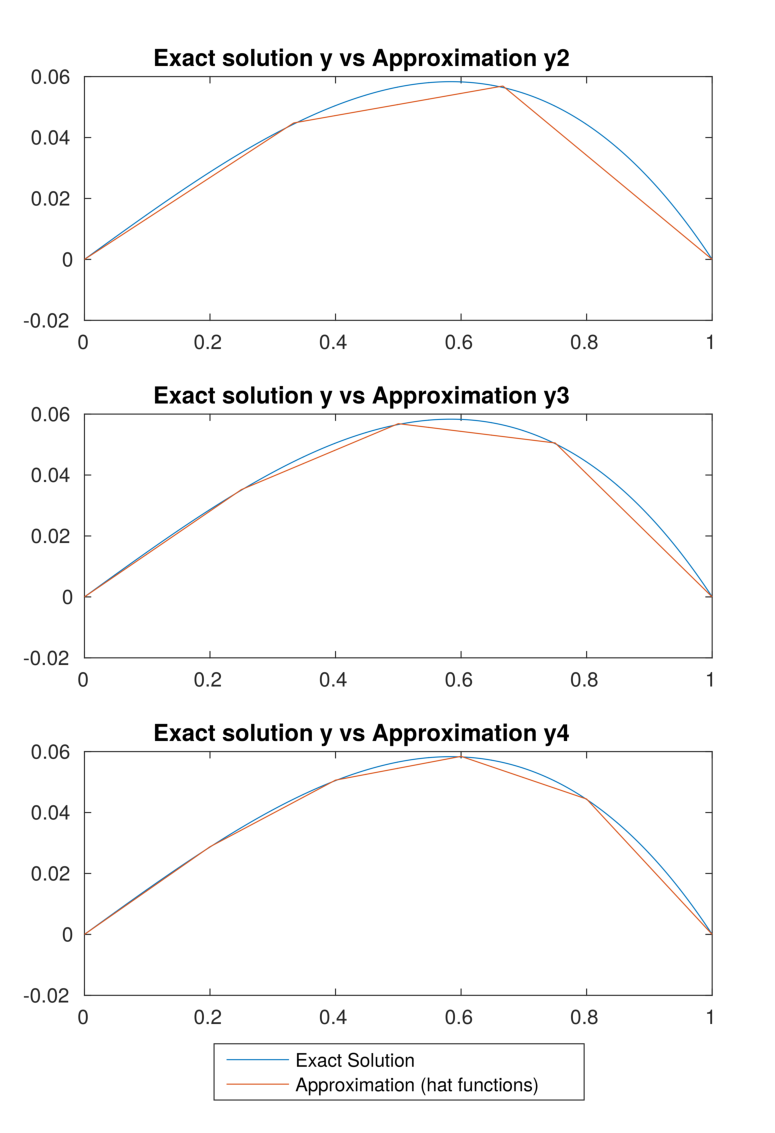
\includegraphics[scale=1.0]{hat_basis_comparison}
    \end{center}
    \caption{Plots of exact solution $y$ and approximation $y_n$ over the interval $[0, 1]$
      using the hat basis.}\label{hat_plot}
  \end{figure}

  The tri-diagonal nature of the coefficient matrix shows that the matrix is sparse.
  MATLAB provides optimized functions for solving systems involving sparse matrices.
  Even though this is not as quick as finding the inverse of a diagonal matrix,
  it is still quite quick in MATLAB. This, coupled with the fact that only at most
  two of the evaluations of the basis functions are needed to compute a point
  on the approximation, shows that this may indeed be the best method for approximating
  the exact solution to this particular differential equation. As such, we have implemented
  special cases of the algorithm for the creation of the coefficient matrix and column vector
  as in the trigonometric basis case.

\end{proof}